% !TEX program = xelatex
\documentclass[a4paper]{exam}
\usepackage{amsmath}
\usepackage{amsthm}
\usepackage[left=1.8cm,right=1.8cm,top=2.2cm,bottom=2.0cm]{geometry}
\usepackage[UTF8]{ctex}
\usepackage{enumerate}
\usepackage{fancyhdr}
\usepackage{xpatch}
\usepackage{graphicx} 
\usepackage{float} 
\usepackage{subfigure} 
\usepackage{amsfonts}
\usepackage{mathtools}
\usepackage{framed}
\usepackage{multicol}
\usepackage{minted}
\usepackage{fontspec}
\usepackage{float}
\usepackage{tikz}
\usepackage{hyperref}
\usepackage{multicol,comment}
\usepackage{biblatex}
\addbibresource{07-discussion.bib}
\usepackage{tikz}

\usetikzlibrary{automata,positioning}
\theoremstyle{definition}
\newtheorem*{solution*}{\textbf{Solution:}}
\newtheorem*{proof*}{\textbf{Proof:}}
\newtheorem{theorem}{Theorem}[subsection]
\newtheorem{definition}{Definition}[subsection]
\newtheorem{lemma}{Lemma}[subsection]
\makeatletter

\AtBeginDocument{\xpatchcmd{\@thm}{\thm@headpunct{.}}{\thm@headpunct{}}{}{}}
\makeatother
\printanswers
\pagestyle{fancy}
\renewcommand{\baselinestretch}{1.15}

\usepackage{paralist}
\let\itemize\compactitem
\let\enditemize\endcompactitem
\let\enumerate\compactenum
\let\endenumerate\endcompactenum
\let\description\compactdesc
\let\enddescription\endcompactdesc

% shorten footnote rule
\xpatchcmd\footnoterule
  {.4\columnwidth}
  {1in}
  {}{\fail}

\title{CS 131 Compilers: Discussion 7: Operational Semantics, Runtime Resourse Allocation and More on Optimization Passes}
\author{\textbf{杨易为}~~\textbf{吴凌云}~~\textbf{樊雨鑫} \\ \texttt{ \{yangyw,wuly2,fanyx\}@shanghaitech.edu.cn}}

\begin{document}
\maketitle
\section{Operational Semantics}
Operational Semantics are optional in defining a language codegen. But the formal definition of the code is to make the code easy to understand and reduce ambiguity. \textbf{Formal Semantics} are unambiguous abstractions of how the program is executed on a machine. They guide the implementation of Code Generators

One kind of Formal Semantics is Operational Semantics (操作语义), where we use Operational Rules to demonstrate the effect of every possible operation. Similar to Type Systems, these rules are in the form of Rules of Inference, but different Contexts are needed, and the thing we infer is Value $v$ instead of Type $T$, along with a new Store.

\begin{enumerate}
    \item  Environment $E: E(x)=l_{x}$ tells the address (location) in memory where $x^{\prime}$ s value is stored
    \begin{enumerate}
        \item e.g. $E=\left[x: l_{x}, y: l_{y}\right]$
        \item Will never change after an operation
    \end{enumerate}
\item Store $S: S\left(l_{x}\right)=v$ tells the value stored in location $l_{x}$
\begin{enumerate}
    \item e.g. $S=\left[l_{x}: 2, l_{y}: 0\right]$
    \item $S\left[v / l_{x}\right]$ means to update $S$ by adding information $S\left(l_{x}\right)=v$
     
     Needed for let / case expressions, since they introduce new variables in new sub-scopes
     \item A Rule may have side effects: change the Store
\end{enumerate}
\item Self-object so: current self object, needed for inferring self
\begin{enumerate}
\item Will never change after an operation
\end{enumerate}

\end{enumerate}
\subsection{COOL Operational Semantics}
Specially for COOL, where everything are Objects, we denote a value as $v=T\left(a_{1}=l_{1}, \ldots, a_{n}=l_{n}\right)$
\begin{enumerate}
    \item $T$ is the Dynamic Type of value $v$
\item $a_{i}$ is the $i$ th Attribute, where the location of $a_{i}$ 's value is $l_{i}$
\item Special notations for basic classes:
\begin{enumerate}
    \item $\operatorname{Int}(5)$ : integer value 5
\item $\operatorname{Bool}($ true): boolean value true
\item $\operatorname{String}(4$, "Cool" $)$ : string "Cool" with length 4
\item void: special instance of all types, only effective for isvoid
\end{enumerate}
\end{enumerate}
Several additional rules are introduced for new objects and method dispatches:
\begin{enumerate}
    \item $l_{\text {new }}=$ newloc $(S)$ means allocate a new, free location $l_{\text {new }}$ in memory
\item Needed for let / case / new expressions, since they ask for new objects
\item Hides some details like the size and strategy of allocation
$D_{T}$ means the default value object of Type $T$
$\operatorname{class}(T)=\left(a_{1}: T_{1} \leftarrow e_{1}, \ldots, a_{n}: T_{n} \leftarrow e_{n}\right)$ illustrates the composition of Type $T$
\begin{enumerate}
   \item Needed for new expressions
\end{enumerate}

\item $\operatorname{impl}(T, f)=\left(e_{1}, \ldots, e_{n}, e_{b o d y}\right)$ illustrates the composition of Method $T . f$
\begin{enumerate}
    \item Needed for method dispatches
\end{enumerate}

\end{enumerate}
\subsection{ChocoPy Operational Semantics}
Specially for ChocoPy, where everything are Objects, we denote a value as $v=X\left(a_{1}=l_{1}, a_{2}=l_{2}, \ldots, a_{n}=l_{n}\right)$
\begin{enumerate}
    \item $X$ is the Class of value $v$
\item $a_{i}$ is the $i$ th Attribute of class $X$, where the location of $a_{i}$ 's value is $l_{i}$
\item Special notations for basic classes:
\begin{enumerate}
    \item $\operatorname{int}(5)$
\item $\operatorname{bool}($ True $)$
\item $\operatorname{str}(7$, "ChocoPy")
\item $v=\left[l_{0}, l_{2}, \ldots, l_{n-1}\right]$
\item $None$
\end{enumerate}
\end{enumerate}
Several additional rules are introduced for new objects and method dispatches:
\begin{enumerate}
  \item newloc same as above
  \item $v=\left(x_{1}, \ldots, x_{n}, y_{1}=e_{1}, \ldots, y_{k}=e_{k}, b_{b o d y}, E_{f}\right)$ for function definitions.
  \item $\operatorname{class}(A)=\left(a_{1}=e_{1}, \ldots, a_{m}=e_{m}\right)$ for class instance
  \item for str / list have different semantics
  \item \begin{aligned}
&\text { The initial and store } G_{i n i t} \text { and } S_{i n i t} \text { hold the predefined functions: }\\
&G_{\text {init }}=\emptyset\left[l_{\text {len }} / \text { len }\right]\left[l_{\text {print }} / \text { print }\right]\left[l_{\text {input }} / \text { input }\right]\\
&S_{\text {init }}\left(l_{\text {print }}\right)=(\text { val, native print, } \emptyset)\\
&S_{\text {init }}\left(l_{l e n}\right)=(\text { val, native len, } \emptyset)\\
&S_{\text {init }}\left(l_{\text {input }}\right)=(\text { native print, } \emptyset)
\end{aligned}
\end{enumerate}

\subsection{C++ Variable Length Array Operational Semantics}
The C programming language\cite{openstd} includes variable-length arrays(VLA) \cite{makinglessdangerous}, a feature where we can allocate an auto array (on stack) of variable size, which was used widely in the Linux Kernel for resource allocation. But because of the tedious translation into the machine code and possible security issue, the recent kernel is VLA-free and C++ is partially abandon it. Therefore, the compiler shall do the semantic check for unacceptable following statements. Extend the typing semantics can be found at C manual 8.1.2 Function calls\cite{cfuncall} and C++ semantics page 7\cite{cs230lec06}, so that the following C++ code will emit a semantic error.
\begin{minted}[mathescape, linenos]{c++}
template<class T>class array{ 
  int s;
  T* elements; 
public:
  array(int n); // allocate "n" elements and let "elements" refer to them 
  array(T* p, int n); // make this array refer to p[0..n-1]
  operator T*(){return elements;}
  int size()const{return s;} 
  // the usual container operations, such as = and [], much like vector 
};

void h(array<double>a); //C++
void g(int m,double vla[m]); //C99
void f(int m,double vla1[m],array<double>a1) {
    array<double> a2(vla1,m); // a2 refers to vla1 
    double*p=a1; //p refers to a1's elements

    g(m,vla1);
    g(a1.size(),a1); // a bit verbose 
    g(a1); //???
}
\end{minted}
The calls marked with ? ? ? cannot be written in C++. Had they gotten past the type checking, the result would have executed correctly because of structural equivalence. If we somehow accept these calls, by a general mechanism or by a special rule for array and VLAs, arrays and VLAs would be completely interchangeable and a programmer could choose whichever style best suited taste and application.
\subsubsection{Semantic of VLA}
We look into 2 codes:
\begin{multicols}{2}
\begin{minted}[mathescape, linenos]{c++}
void call_me(char *stuff, int step) {
  char buf [10];
  strlcpy(buf, stuff, sizeof(buf));
  printf("%d: [%s] \n", step, buf);
}
\end{minted}

We \href{https://godbolt.org/z/498csxnhK}{have}:
\begin{minted}[mathescape,linenos]{c++}
        push    rbp
        mov     rbp, rsp
        sub     rsp, 32
        mov     QWORD PTR [rbp-24], rdi
        mov     DWORD PTR [rbp-28], esi
        mov     rcx, QWORD PTR [rbp-24]
        lea     rax, [rbp-10]
        mov     edx, 10
        mov     rsi, rcx
        mov     rdi, rax
        mov     eax, 0
        call    strlcpy
        lea     rdx, [rbp-10]
        mov     eax, DWORD PTR [rbp-28]
        mov     esi, eax
        mov     edi, OFFSET FLAT:.LC0
        mov     eax, 0
        call    printf
        nop
        leave
        ret
\end{minted}
For the \href{https://godbolt.org/z/fx5oKqaeE}{variable length array}.
\begin{minted}[mathescape,linenos]{c++}
void call_me(char *stuff, int step) {
  char buf [step];
  strlcpy(buf, stuff, sizeof(buf));
  printf("%d: [%s] \n", step, buf);
}
\end{minted}
\begin{minted}[mathescape,linenos]{c++}
        push    rbp
        mov     rbp, rsp
        push    rbx
        sub     rsp, 56
        mov     QWORD PTR [rbp-40], rdi
        mov     DWORD PTR [rbp-44], esi
        mov     rax, rsp
        mov     rbx, rax
        mov     ecx, DWORD PTR [rbp-44]
        movsx   rax, ecx
        sub     rax, 1
        mov     QWORD PTR [rbp-24], rax
        movsx   rax, ecx
        mov     r10, rax
        mov     r11d, 0
        movsx   rax, ecx
        mov     r8, rax
        mov     r9d, 0
        movsx   rax, ecx
        mov     edx, 16
        sub     rdx, 1
        add     rax, rdx
        mov     QWORD PTR [rbp-56], 16
        mov     edx, 0
        div     QWORD PTR [rbp-56]
        imul    rax, rax, 16
        sub     rsp, rax
        mov     rax, rsp
        add     rax, 0
        mov     QWORD PTR [rbp-32], rax
        movsx   rdx, ecx
        mov     rax, QWORD PTR [rbp-32]
        mov     rcx, QWORD PTR [rbp-40]
        mov     rsi, rcx
        mov     rdi, rax
        mov     eax, 0
        call    strlcpy
        mov     rdx, QWORD PTR [rbp-32]
        mov     eax, DWORD PTR [rbp-44]
        mov     esi, eax
        mov     edi, OFFSET FLAT:.LC0
        mov     eax, 0
        call    printf
        mov     rsp, rbx
        nop
        mov     rbx, QWORD PTR [rbp-8]
        leave
        ret
\end{minted}
\end{multicols}
\subsubsection{Semantic of Multi-dimensional Array}
\begin{enumerate}
    \item One-dimensional Arrays
    
    How do we process retrieval from and assignment to $x[i]$, for an array $x$ ?
\begin{solution}
We assume that all items of the array have fixed size-S bytes and are arranged sequentially in memory (the usual representation).
Easy to see that the address of $x[i]$ must be
$$
\& x+S \cdot i
$$
where \& $\mathrm{x}$ is intended to denote the address of the beginning of $\mathrm{x}$. Generically, we call such formulae for getting an element of a data structure access algorithms.
The IL might look like this:
$\begin{aligned} t_{0}=& \operatorname{cgen}\left(\& \mathrm{~A}[\mathrm{E}], t_{0}\right): \\ & t_{1}=\operatorname{cgen}(\& \mathrm{~A}) \\ & t_{2}=\operatorname{cgen}(\mathrm{E}) \\ \Rightarrow & t_{3}:=t_{2} * \mathrm{~S} \\ \Rightarrow & t_{0}:=t_{1}+t_{3} \end{aligned}$
\end{solution}
\item Multi-dimensional  Arrays
\begin{enumerate}
    \\  A 2D array is a 1D array of $1 D$ arrays.
   \\ Java uses arrays of pointers to arrays for $>1 D$ arrays.
\\ But if row size constant, for faster access and compactness, may prefer to represent an $M \times N$ array as a 1D array of $M$ 1D rows of length $N$ (not pointers to rows): row-major order...
\\ Or, as in FORTRAN, a 1D array of $N 1 D$ columns of length $M$ : column-major order.
\\ So apply the formula for 1D arrays repeatedly-first to compute the beginning of a row and then to compute the column within that row:
$$
\& A[i][j]=\& A+i \cdot S \cdot N+j \cdot S
$$
for an M-row by N-column array stored in column-major order.
\\ Where does this come from? Assuming S, again, is the size of an individual element, the size of a row of $N$ elements will be $S \cdot N$.
\\
$\begin{aligned} t=& \text { cgen }(\& e 1[e 2, e 3]): \\ & \# \text { Compute e1, e2, e3, and } \mathrm{N}: \\ & \text { t1 }=\operatorname{cgen}(\mathrm{e} 1) ; \\ & \text { t2 }=\operatorname{cgen}(\mathrm{e} 2) ; \\ & \text { t3 }=\operatorname{cgen}(\mathrm{e} 3) \\ & \text { t4 }=\operatorname{cgen}(\mathrm{N}) \# \text { (N need not be constant) } \\ & \Rightarrow t 5:=t 4 * t 2 \\ & \Rightarrow t 6:=\text { t5 }+\text { t3 } \\ & \Rightarrow t 7:=\text { t6 } * \mathrm{~S} \\ & \Rightarrow t:=t 7+t 1 \\ & \text { return } t \end{aligned}$
\end{enumerate}
\item Array Descriptors
\begin{enumerate}
    \item Calculation of element address \&e1 $[\mathrm{e} 2, \mathrm{e} 3]$ has the form
$$V O+S 1 \times e 2+52 \times e 3$$
where
\\ VO (\&e1 $[0,0])$ is the virtual origin.
\\ S1 and S2 are strides.
\\ All three of these are constant throughout the lifetime of the array (assuming arrays of constant size).
\item Therefore, we can package these up into an array descriptor, which can be passed in lieu of a pointer to the array itself, as a kind of "fat pointer" to the array:
$$\begin{tabular}{|c|c|c|}
\hline$\& \mathrm{\& e}[0][0]$ & $\mathrm{S} \times \mathrm{N}$ & $\mathrm{S}$ \\
\hline
\end{tabular}$$
\item Assuming thate1now evaluates to the address of a 2D array de-scriptor, the IL code becomes:
$t=\operatorname{cgen}(\operatorname{se1}[\mathrm{e} 2, \mathrm{e} 3]):$\\
$\mathrm{t} 1=\operatorname{cgen}(\mathrm{e} 1) ; \quad \#$ Yields a pointer to a descriptor.\\
$t 2=\operatorname{cgen}(\mathrm{e} 2 ;$\\
t3 $=\operatorname{cgen}(\mathrm{e} 3)$\\
$\Rightarrow$ t4 := *t1; # The VO\\
$\Rightarrow$ t5 :=*(t1+4) # Stride #1\\
$\Rightarrow$ t6 :=*(t1+8) # Stride #2\\
$\Rightarrow$ t7 $:=$ t5 $*$ t2\\
$\Rightarrow$ t8 := t6 $*$ t3\\
$\Rightarrow \mathrm{t} 9:=\mathrm{t} 4+\mathrm{t} 7$\\
$\Rightarrow t 10:=t 9+t 8$

\item By judicious choice of descriptor values, can make the same formula work for different kinds of array.
\\ For example, if lower bounds of indices are 1 rather than 0 , must compute address
\&e $[1,1]+\mathrm{S} 1 \times(\mathrm{e} 2-1)+\mathrm{S} 2 \times(\mathrm{e} 3-1)$
\\ But some algebra puts this into the form
$$
\mathrm{VO}^{\prime}+\mathrm{S} 1 \times \mathrm{e} 2+\mathrm{S} 2 \times \mathrm{e} 3
$$
where
$$
\text { VO' }=\& \mathrm{e}[1,1]-\mathrm{S} 1-\mathrm{S} 2=\& \mathrm{e}[0,0] \text { (if it existed). }
$$
\\ So with the descriptor
$$\begin{tabular}{|c|c|c|}
\hline VO' & $\mathrm{S} \times \mathrm{N}$ & $\mathrm{S}$ \\
\hline
\end{tabular}$$
we can use the same code as on the last slide.
\\By passing descriptors as array parameters, we can have functions that adapt to many different array layouts automatically.
\item Other Uses  for  Descriptors\\
No reason to stop with strides and virtual origins: can include other data.
\\By adding upper and lower index bounds to a descriptor, can easily implement bounds checking.
\\This also allows for runtime queries of array sizes and bounds.
\\Descriptors also allow views of arrays: nothing prevents multiple descriptors from pointing to the same data.
\\This allows effects such as slicing, array reversal, or array transposition without copying data.
\\ Example:
Consider a simple base array (in $C$ ):
\begin{minted}[mathescape,linenos]{c}
int data [12]={1,2,3,4,5,6,7,8,9,10,11,12};
\end{minted}
and descriptor types (including lengths):
\begin{minted}[mathescape,linenos]{c}
struct Desc1 { int* VO, int S1, int len1 };
struct Desc2 { int* V0, int S1, int len1, int S2, int len2 };
\end{minted}
Here are some views
\begin{minted}[mathescape,linenos]{c}
Desc1 v0 = { data, 4, 12 }; /* All of data. */
Desc1 v1 = { &data[3], 4, 3 }; /* data[3:6]: [4, 5, 6]. */
/* Every other element of data: [1, 3, ...] */
Desc1 v2 = { data, 8, 6 };Desc1 v3 = { &data[11], -4, 12 };
/* Reversed: [12, 11, ...] */

/* As a 2D 4x3 array: [ [ 1, 2, 3 ], [ 4, 5, 6 ], ... ] */
Desc2 v4 = { data, 12, 4, 4, 3 };
/* As row 2 of v4: [7, 8, 9] */
Desc1 v5 = { &data[6], 4, 3 }
\end{minted}
\end{enumerate}
\end{enumerate}
\section{Runtime System}
The \textbf{Runtime System (Environment)} defines the way of managing run-time resources. It depends largely on the machine architecture and OS.

\begin{enumerate}
    \item Memory Layout and Usage:
\begin{enumerate}
    \item Allocation and Layout of objects
    \item Function call strategies
    \item Garbage collection or not, and how
\end{enumerate}
\item Convention of using Registers
\item Runtime Error handling API
\begin{enumerate}
    \item Dispatch on void: design of Type System has flaws
\item Division on zero (除零错误): we can hardly know what is the exact dynamic \item value of a denominator at compile-time Case match failed on all branches
\end{enumerate}
\end{enumerate}
To generate workable code, we MUST obey uniform routines with the Runtime System definitions when implementing the Code Generator. Thus, Code Generator design MUST consider the run-time requirements of the target machine and OS.


For the detailed COOL Runtime System Conventions, refer to COOL Runtime System, section 2-5.
\begin{enumerate}
    \item  In object layouts, subclasses arrange its attributes from the oldest ancestor's (i.e. object) down to its private ones
 \item In dispatch tables, subclasses arrange its methods similarly, but whenever a method is shadowed, will dispatch on the one of the closest parent's (may be himself)
\end{enumerate}
\subsection{Activation}
An Activation is an invocation of a procedure / function. Its lifetime lasts until the last step of execution of that procedure,
\begin{enumerate}
    \item For two different activations $a, b$, their lifetimes are either  Non-overlapping or Nested 
     \item An Activation is a particular instance of the function's invocation 
      \item Sequence of function calls represented as an Activation Tree
      \begin{enumerate}
      \item e.g.
      \begin{figure}[htbp]
  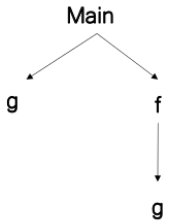
\includegraphics[width=2cm]{./img/main_activation.png}
\end{figure}
          \item Earlier Activation goes on the left
      \end{enumerate}
\end{enumerate}
A Stack can be used to track current Activations, which is a common practice in modern Languages. On each invocation, an Activation Record is pushed onto the stack. It is popped out when the procedure ends.

The design of Activation Records is an important part of the Runtime System, e.g.
\begin{figure}[htbp]
  \centering
  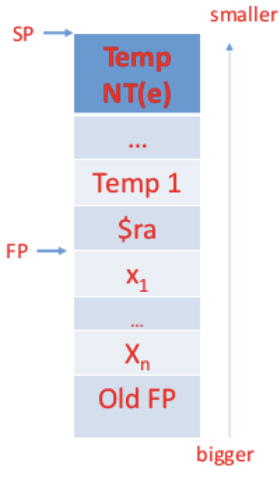
\includegraphics[width=5cm]{./img/fp_sp.png}
\end{figure}
\begin{enumerate}
    \item What needs to be inside an Activation Record
    \item Their exact layouts
 \item Caller / Callee is responsible for which part
\end{enumerate}
\section{More on Optimization Passes}
\subsection{Vectorization\cite{llvmautovec} \cite{cornellllvmautovec}}
Let dive into the following two cases:
\begin{minted}[mathescape,linenos]{python}
def test_vec(a: int, b: int, c: int, d: int, e: int, f: int, g: int, h: int, x: int) -> int:
    if x > 0:
        a = e + 4
        b = f + 4
        c = g + 4
        d = h + 4
    return a + b + c + d
print(test_vec(1, 2, 3, 4, 5, 6, 7, 8, 9))
\end{minted}
and 
\begin{minted}[mathescape,linenos]{python}
def test() -> int:
    a: [int] = None
    i: int = 0
    a = [1, 2, 3, 4, 1, 2, 3, 4]
    for i in [1, 2, 3, 4, 5, 6, 7, 8]:
        a[i] = a[i] + 1
    return a[0]
print(test())
\end{minted}
Both of the array for loop access and different variable doing the same operator can be vectorized. We first have to identify the pattern with \texttt{Loopfind} using the strong connectivity algorithm which will be covered next class. and then check the bound and the inductive varible are valid, lastly using \texttt{insertelement} and \texttt{extractelement} to let them scalarize and do the vector operations.
\subsection{Multithread}
具体过程:find + wrap

\hypertarget{find}{%
\paragraph{find}\label{find}}

find的条件很多,简而言之,找到每个最内循环的最外层循环,然后看能否\texttt{MultiThreading}化

这个外层循环应该满足的条件是:

\begin{itemize}
\item
  需要一个start到end的递增模式
\item
  分支指令应该是\texttt{Br\ Lt\ i32\ Const\ \textless{}Label1\textgreater{}\ \textless{}Label2\textgreater{}}的形式
\item
  不能有其他Phi指令(迷,这样就限制了只能有一个循环变量
\end{itemize}

以矩阵赋值的例子,br是根据 i 和 n 的大小关系

Phi的四个操作数

\begin{enumerate}
\def\labelenumi{\arabic{enumi}.}
\item
  i、递增变量
\item
  BB1、递增 i 的BB
\item
  Constant、100,循环边界
\item
  BB2、\%entry
\end{enumerate}

累加值:

\begin{minted}[mathescape,linenos]{c}
auto accuVal = dynamic_cast<ConstantInt *>(accu->getOperand(1));
\end{minted}

\hypertarget{wrap}{%
\paragraph{wrap}\label{wrap}}

包装部分:在循环的条件Block之前插入ACCstart,在更新迭代变量的之前插入ACCend

\begin{minted}[mathescape,linenos]{c}
while (i<n){
	A[i] = A[i]+B[i];
}
\end{minted}

插入多线程部分之前

\begin{figure}[htbp]
  \centering
  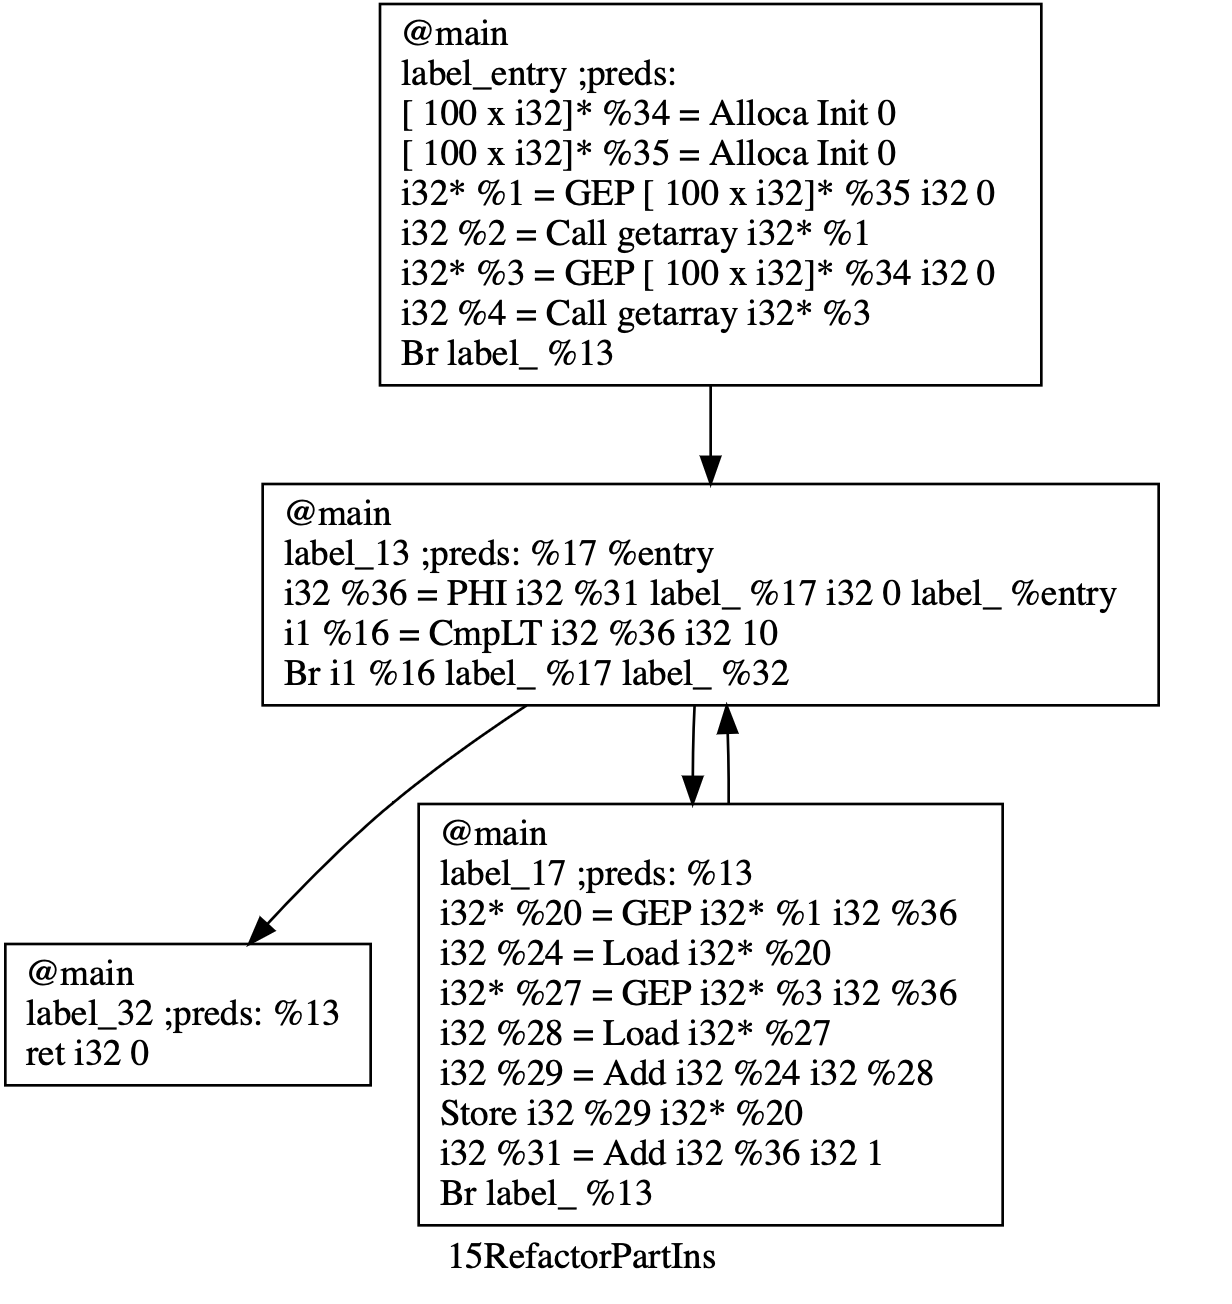
\includegraphics[width=5cm]{./img/0.png}
\end{figure}

插入之后:

\begin{minted}[mathescape,linenos]{llvm}
%37: 多线程号 tid
%38: 问题规模 n
%40: _l = (n*tid)/4 
%43: _r = (n*(tid+1))/4
%44: _r + start		右边界
%48: (_l + step-1)/step * step + start		迭代变量初始值
\end{minted}

\begin{figure}[htbp]
  \centering
  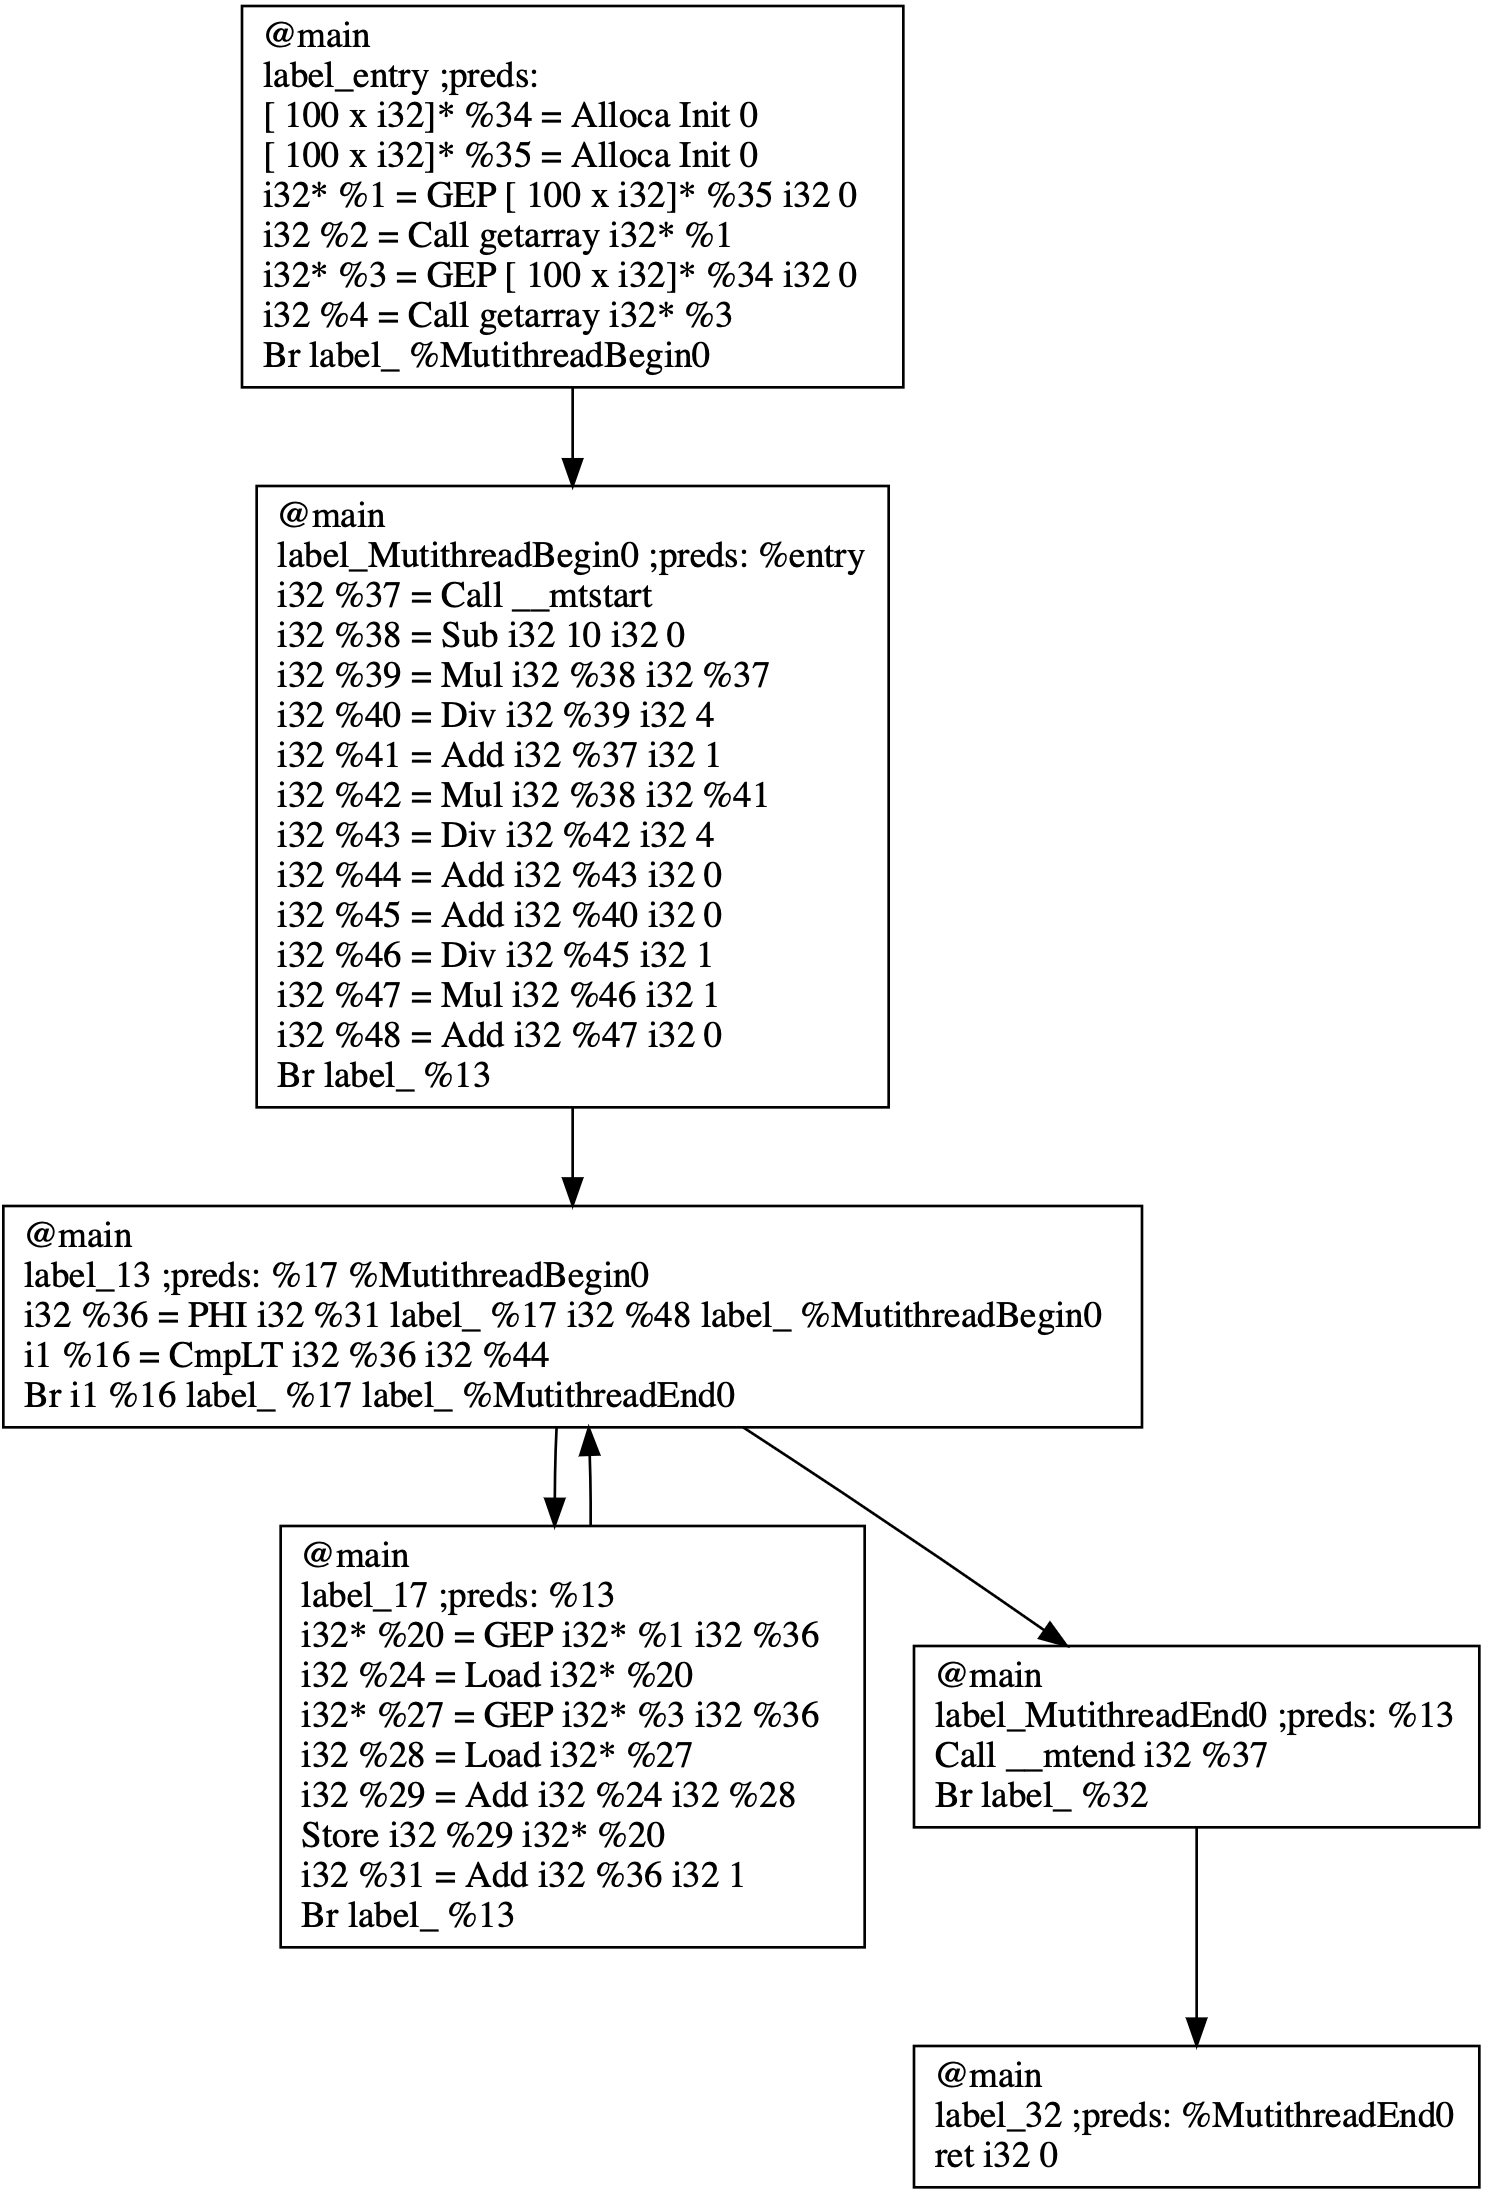
\includegraphics[width=5cm]{./img/1.png}
\end{figure}

\begin{minted}[mathescape,linenos]{llvm}
define @main()
<label>entry:   level=0   preds=   succs=(%13)
    REG 4    [ 100 x i32]* %34  = Alloca 
    REG 1    [ 100 x i32]* %35  = Alloca 
    REG 0    i32 %2  = Call getarray [ 100 x i32]* %35 
    REG 0    i32 %4  = Call getarray [ 100 x i32]* %34 
    REG 10    i32 %37  = Call accstart 
 MT REG 2    i32 %39  = Mul i32 10 i32 %37 
 MT REG 0    i32 %41  = Add i32 %37 i32 1 
 MT REG 0    i32 %42  = Mul i32 10 i32 %41 
 MT REG 5    i32 %50  = AShr i32 %42 i32 2 
 MT REG 0    i32 %51  = AShr i32 %39 i32 2 
 MT REG 0    i32 %52  = Shl i32 %51 i32 0 
 MT          Br <label> %13 
<label>13:   level=1   preds=(%17 %entry)   succs=(%17 %MutithreadEnd0)
 MT REG 0    i32 %36  = PHI i32 %31 <label> %17 i32 %52 <label> %entry 
 MT          Br LT i32 %36 i32 %50 <label> %17 <label> %MutithreadEnd0 
<label>17:   level=1   preds=(%13)   succs=(%13)
 MT REG 3    i32 %24  = Load [ 100 x i32]* %35 i32 %36 i32 2 
 MT REG 2    i32 %28  = Load [ 100 x i32]* %34 i32 %36 i32 2 
 MT REG 2    i32 %29  = Add i32 %24 i32 %28 
 MT          Store i32 %29 [ 100 x i32]* %35 i32 %36 i32 2 
 MT REG 0    i32 %31  = Add i32 %36 i32 1 
 MT          Br <label> %13 
<label>MutithreadEnd0:   level=0   preds=(%13)   succs=
             Call accend i32 %37 
             ret i32 0 
\end{minted}
首先知道system call的约定

\begin{minted}[mathescape,linenos]{rst}
> man syscall 2
The first table lists the instruction used to transition to kernel
mode, the register used to indicate the system call number, the 
register used to return the sys‐tem call result, and the register 
used to signal an error.

arch/ABI    instruction           syscall #  retval  error    Notes
────────────────────────────────────────────────────────────────────
arc         trap0                 r8         r0      -
arm/OABI    swi NR                -          a1      -        [2]
arm/EABI    swi 0x0               r7         r0      -
arm64       svc #0                x8         x0      -
riscv       ecall                 a7         a0      a1        -

Note:
[2] NR is the system call number.

The second table shows the registers used to pass the system call
arguments.

arch/ABI      arg1  arg2  arg3  arg4  arg5  arg6  arg7  Notes
──────────────────────────────────────────────────────────────
arc           r0    r1    r2    r3    r4    r5    -
arm/OABI      a1    a2    a3    a4    v1    v2    v3
arm/EABI      r0    r1    r2    r3    r4    r5    r6
arm64         x0    x1    x2    x3    x4    x5    -
riscv         a0    a1    a2    a3    a4    a5    -
\end{minted}

然后man clone 2

\begin{minted}[mathescape,linenos]{c}
int clone(int (*fn)(void *), void *stack, int flags, void *arg, ...
          /* pid_t *parent_tid, void *tls, pid_t *child_tid */ );
\end{minted}

Linux对线程的设计:线程只不过是共享虚拟地址空间和文件描述符表的进程,定义上线程之间共享除寄存器、栈、线程内本地存储(thread-local
storage, TLS)之外的所有东西。

操作系统和底层硬件天然地保证了线程不会共享寄存器,TLS
不是必须的,本项目又使得线程之间共享栈空间,所以几乎没有切换开销

clone跟fork都是创建子进程(线程),区别在于clone能更详细的定制子进程和父进程共享的内容:如虚拟内存地址空间,文件描述符表,the
table of signal handlers

clone对父进程返回所创建的子进程的tid,如果失败,返回-1

\texttt{clone\_flags}的长度为8个字节,减去发送给父进程的信号代码的一个字节后剩下了7个字节用于传递进程复制信息,即可以同时设置7*8=56个标志位,也就是可以同时控制24种进程信息的复制。要设置某个标志位时只需要将其对应的取值与\texttt{clone\_flags}进行或运算即可:

为啥clone\_flags是273

273的32位二进制是0000000100010001,十六进制0x0111

\href{https://elixir.bootlin.com/linux/v5.17/source/include/uapi/asm-generic/signal.h\#L18}{linux
5.17 sched.h}

\begin{minted}[mathescape,linenos]{c}
/*
 * cloning flags:
 */
#define CSIGNAL		0x000000ff	/* signal mask to be sent at exit */
#define CLONE_VM	0x00000100	/* set if VM shared between processes */
#define CLONE_FS	0x00000200	/* set if fs info shared between processes */
#define CLONE_FILES	0x00000400	/* set if open files shared between processes */
/*....*/
#define CLONE_NEWUSER		0x10000000	/* New user namespace */
#define CLONE_NEWPID		0x20000000	/* New pid namespace */
#define CLONE_NEWNET		0x40000000	/* New network namespace */
#define CLONE_IO		0x80000000	/* Clone io context */
\end{minted}

在
\href{https://elixir.bootlin.com/linux/v5.17/source/kernel/fork.c\#L2502}{kernel/fork.c}

\begin{minted}[mathescape,linenos]{c}
/* ok, now we should be set up.. */
p->exit_signal = (clone_flags & CLONE_THREAD) ? -1 : (clone_flags & CSIGNAL);
p->pdeath_signal = 0;
p->exit_state = 0;
\end{minted}
至于为啥最后两个数字是17

定义在
\href{https://elixir.bootlin.com/linux/v5.17/source/include/uapi/asm-generic/signal.h\#L18}{include/uapi/asm-generic/signal.h}
32个信号量
\begin{minted}[mathescape,linenos]{c}
#define SIGHUP		 1
#define SIGINT		 2
#define SIGQUIT		 3
#define SIGILL		 4
#define SIGTRAP		 5
#define SIGABRT		 6
#define SIGIOT		 6
#define SIGBUS		 7
#define SIGFPE		 8
#define SIGKILL		 9
#define SIGUSR1		10
#define SIGSEGV		11
#define SIGUSR2		12
#define SIGPIPE		13
#define SIGALRM		14
#define SIGTERM		15
#define SIGSTKFLT	16
#define SIGCHLD		17
//...
\end{minted}

项目默认关闭多线程优化Pass

与经典框架 OpenMP 对比的优点

\begin{itemize}
\item
  节约了栈开销:不需要将被并行化的区域拆分出来变成函数
\item
  节约了切换上下文:不需要保存上下文和维护各种信息
\item
  仅仅需要维护线程独有的寄存器
\end{itemize}

\hypertarget{accstart}{%
\paragraph{accstart}\label{accstart}}

\begin{minted}[mathescape,linenos]{bash}
# Runtime support function accstart
  mv fp, sp
  add t1, zero, zero
  lui t1, 1044480
  add sp, sp, t1
  add sp, sp, -12
  sw  a0, 0(sp)
  sw  a1, 4(sp)
  sw  a2, 8(sp)
  sw  a3, 12(sp)
  mv a3, a7
  addi a2, zero, 4
accstart_1:
  addi a2, a2, -1
  beqz a2, accstart_2
  addi a7, zero, 120
  addi a0, zero, 20
  mv a1, sp
  ecall
  bnez a0, accstart_1
accstart_2:
  mv tp, a2
  mv a7, a3
  lw  a0, 0(sp)
  lw  a1, 4(sp)
  lw  a2, 8(sp)
  lw  a3, 12(sp)
  add sp, sp, 12
  add s1, zero, zero
  lui s1, 4096
  add sp, sp, s1
  ret
\end{minted}
\hypertarget{accend}{%
\paragraph{accend}\label{accend}}
\begin{minted}[mathescape,linenos]{bash}
# Runtime support function accend
  beqz s1, .accend_2
.accend_1:
  call exit
.accend_2:
  addi sp, sp, -16
  sw  a0, 0(sp)
  sw  a1, 4(sp)
  sw  a2, 8(sp)
  sw  a3, 12(sp)
  addi a1, zero, 4
.accend_3:
  addi a1, a1, -1
  beqz a1, .accend_4
  addi sp, sp, -8
  sw  a1, 0(sp)
  sw  ra, 4(sp)
  addi sp, sp, -4
  mv a0, sp
  jal wait
  addi sp, sp, 4
  lw  a1, 0(sp)
  lw  ra, 4(sp)
  addi sp, sp, 8
  j .accend_3
.accend_4:
  lw  a0, 0(sp)
  lw  a1, 4(sp)
  lw  a2, 8(sp)
  lw  a3, 12(sp)
  addi sp, sp, 16
  mv s1, zero
  ret
\end{minted}
\printbibliography
\end{document}
